% =============================================================================
% Artigo final de PLN (UFRGS) — Reranqueamento de passagens em português
% Modelo SBC. Compilação: pdflatex -> bibtex -> pdflatex -> pdflatex
% Números: phase2/results/*.csv e phase2/RESULTS.md (execução de 2026-11-25/26).
% =============================================================================
\documentclass[12pt]{article}

\usepackage{sbc-template}
\usepackage{graphicx,url}
\usepackage[utf8]{inputenc}
\usepackage[T1]{fontenc}
\usepackage[english,brazilian]{babel}
\usepackage{booktabs}
\usepackage{placeins}
\usepackage{amsmath,amssymb}

\graphicspath{{figures/}}
\sloppy

\title{Reranqueamento de Passagens em Português com Cross-Encoders:\\
Ajuste Fino, Cascata e Fusão no mMARCO}

% TODO(autores): preencher nomes, instituição e e-mails.
\author{TODO: Autor Um\inst{1}, TODO: Autor Dois\inst{1}}

\address{Instituto de Informática -- Universidade Federal do Rio Grande do Sul (UFRGS)\\
  Porto Alegre -- RS -- Brasil
  \email{\{todo.autor1,todo.autor2\}@inf.ufrgs.br}
}

\begin{document}

\maketitle

\begin{abstract}
This work studies passage reranking for Portuguese with cross-encoders on mMARCO. We show that the evaluation protocol changes the conclusions:
evaluating on training queries over a small corpus with random distractors inflated the
results 3.2 times compared with the official protocol. Under the corrected protocol, a
cross-encoder fine-tuned by us on a free GPU achieves 77\% of the gain of a published
reranker over BM25. We then extend the pipeline with a third stage based on monoPTT5 and
with score fusion: the third stage compensates for a weaker reranker but does not improve
a strong one, while fusing two rerankers of similar strength and different architectures
gives the best result (MRR@10 of 0.292). First-stage retrieval is the main bottleneck, and
reranking helps most when answers share few words with the question.
\end{abstract}

\begin{resumo}
Estudamos o reranqueamento de passagens em português com cross-encoders no mMARCO.
Avaliar com perguntas de treino sobre um corpus pequeno, com distratores aleatórios, inflou
os resultados em 3,2 vezes em relação ao protocolo oficial. Neste, um cross-encoder
ajustado por nós numa GPU gratuita alcança 77\% do ganho de um reranqueador publicado
sobre o BM25. Um terceiro estágio com o monoPTT5 compensa um reranqueador mais fraco, mas
não melhora um forte; já a fusão de dois reranqueadores de força parecida e arquiteturas
diferentes produz o melhor resultado (MRR@10 de 0,292). O primeiro estágio é o principal gargalo, e o reranqueamento ajuda mais
quando a resposta compartilha poucas palavras com a pergunta.
\end{resumo}

% =============================================================================
\section{Introdução}
\label{sec:intro}

Sistemas de busca precisam devolver, entre milhões de textos, os poucos que respondem a uma
pergunta, e precisam fazê-lo \emph{em ordem}: uma resposta correta na quadragésima posição
equivale, na prática, a não encontrá-la. Métodos léxicos como o BM25~\cite{robertson:2009}
são rápidos e robustos, mas só recompensam palavras em comum entre pergunta e texto. Eles
falham com sinônimos (\textit{ACL} e \textit{LCA}), com respostas que não repetem os termos da
pergunta (uma data para uma pergunta com \textit{quando}) e com textos que repetem os termos
mas tratam de outro assunto.

Modelos baseados em Transformers~\cite{vaswani:2017} resolvem parte desse problema ao
representar o significado em contexto. Entre eles, o \emph{cross-encoder} lê pergunta e
passagem juntas e estima a relevância do par; é o modelo mais preciso, mas também o mais
caro, e por isso é usado como segundo estágio, reordenando apenas as candidatas de um
primeiro estágio barato~\cite{nogueira:2019,nogueira:2019multistage}. Para o português, o
mMARCO~\cite{bonifacio:2021} disponibiliza uma tradução automática do MS
MARCO com rótulos de relevância, o que permite treinar e avaliar
reranqueadores na língua.

Nosso objetivo é implementar e avaliar um cross-encoder para reordenar passagens em
português, explorando sua capacidade de cruzar o contexto da pergunta com o das possíveis
respostas. Um primeiro experimento, com uma subamostra do mMARCO montada a partir de
perguntas de treino, indicou MRR@10 de 0,91, um valor três vezes acima do publicado. Investigar
essa discrepância levou às seguintes questões de pesquisa:

\begin{itemize}
  \item \textbf{QP1:} Quanto um cross-encoder ajustado por nós, com orçamento de uma GPU
  gratuita, ganha sobre o BM25 em comparação com um reranqueador publicado?
  \item \textbf{QP2:} Quanto o protocolo de avaliação altera as conclusões?
  \item \textbf{QP3:} Um terceiro estágio e a fusão de pontuações melhoram o resultado, e a
  que custo?
  \item \textbf{QP4:} Que tipos de pergunta mais se beneficiam do reranqueamento?
\end{itemize}

As contribuições são: (i) a quantificação de como vazamento de dados e um corpus fácil
inflam a avaliação; (ii) um cross-encoder treinado com um laço de treinamento próprio, com
curva de aprendizado; (iii) uma comparação passo a passo de um pipeline em três estágios,
incluindo custo de latência e fusão de pontuações; e (iv) uma análise do ganho por tipo de
pergunta. A Seção~\ref{sec:teoria} apresenta os conceitos; a Seção~\ref{sec:relacionados},
os trabalhos relacionados; a Seção~\ref{sec:metodo}, a metodologia; a
Seção~\ref{sec:resultados}, os resultados; e a Seção~\ref{sec:conclusao} conclui.

% =============================================================================
\section{Referencial Teórico}
\label{sec:teoria}

\textbf{BM25.} Função de pontuação léxica~\cite{robertson:2009} baseada nas palavras em comum
entre pergunta e passagem. É rápida e robusta, mas não reconhece sinônimos nem paráfrases.

\textbf{Transformers.} Modelos baseados em autoatenção~\cite{vaswani:2017}, que geram
representações dependentes do contexto. São pré-treinados em grandes volumes de texto e
ajustados (\textit{fine-tuning}) para tarefas específicas.

\textbf{Cross-encoders.} Recebem pergunta e passagem numa única entrada e produzem uma
pontuação de relevância para o par. São mais precisos que modelos que codificam os textos
separadamente (\textit{bi-encoders}), mas caros demais para a coleção inteira; por isso
reordenam apenas as candidatas de um primeiro estágio~\cite{nogueira:2019}.

\textbf{monoT5 e monoPTT5.} Reranqueadores generativos que respondem se a passagem é
relevante; a pontuação é a confiança na resposta positiva. O
monoPTT5~\cite{piau:2024} é a versão para o português do monoT5.

\textbf{Multiestágio e fusão.} Estágios cada vez mais caros podem ser encadeados sobre cada
vez menos candidatas~\cite{nogueira:2019multistage}. Alternativamente, as pontuações de dois
modelos podem ser combinadas, por interpolação ponderada ou por \textit{Reciprocal Rank
Fusion} (RRF)~\cite{cormack:2009}, que usa apenas as posições nos rankings.

\textbf{Métricas.} O MRR@10, métrica oficial do MS MARCO, mede a posição da primeira passagem
relevante no top-10. O nDCG@10 considera todas as relevantes do top-10, e o Recall@$K$, a
fração delas entre as $K$ primeiras. O Recall@$K$ do primeiro estágio é o teto de qualquer
reranqueador que receba $K$ candidatas.

% =============================================================================
\section{Trabalhos Relacionados}
\label{sec:relacionados}

\cite{nogueira:2019} foram os primeiros a usar o BERT para reordenar passagens. No MS MARCO,
reordenando as 1.000 primeiras passagens do BM25, o MRR@10 subiu de 0,167 para 0,365. Em
seguida, \cite{nogueira:2019multistage} propuseram um pipeline em três estágios (BM25,
monoBERT e duoBERT), com MRR@10 de 0,187, 0,372 e 0,390, e mostraram que o número de
candidatas em cada estágio controla o equilíbrio entre qualidade e tempo de resposta. O
protocolo padrão desses trabalhos é treinar com as triplas de treino do MS MARCO e avaliar
no conjunto dev, o mesmo que adotamos aqui.

Para o português, o mMARCO~\cite{bonifacio:2021} traduziu o MS MARCO e obteve MRR@10 de 0,152
com o BM25, 0,289 com um mMiniLM e 0,302 com um mT5. O ptt5-v2~\cite{piau:2024} treinou modelos
T5 em português e, a partir deles, os reranqueadores monoPTT5, chegando a 0,332 com o maior
modelo. \cite{miyaji:2026} mostraram que ajustar com dados escritos originalmente em português,
em vez de traduzidos, melhora o nDCG em até 5 pontos percentuais.

Esses trabalhos treinam com dezenas de milhões de pares em hardware dedicado. Nosso foco é
diferente: o que se consegue com uma GPU gratuita, como o protocolo de avaliação muda as
conclusões, quanto custa cada estágio a mais e em que perguntas o reranqueamento ajuda.

% =============================================================================
\section{Metodologia}
\label{sec:metodo}

\subsection{Conjunto de dados}

Usamos o mMARCO em português~\cite{bonifacio:2021}:
\begin{itemize}
  \item \textbf{Coleção:} 8,8 milhões de passagens.
  \item \textbf{Avaliação:} o conjunto oficial \textit{dev small}, com 6.980 perguntas e,
  em média, uma passagem relevante marcada por pergunta.
  \item \textbf{Treino:} triplas (pergunta, passagem relevante, passagem não relevante). O
  arquivo oficial tem 39,8 milhões; as passagens não relevantes vêm do BM25, ou seja,
  parecem relevantes mas não são (\emph{negativos difíceis}). Sorteamos 302 mil triplas
  (semente 42) e separamos 2 mil para validação.
\end{itemize}

\textbf{Limpeza do texto.} Parte da coleção tem caracteres corrompidos
(\textit{mojibake}). Tentamos corrigi-los com a biblioteca ftfy, que alterou 61.895
passagens e nenhuma pergunta. Analisando as 50 trocas mais frequentes numa amostra de 300 mil
passagens, o reparo foi só parcial. Cerca de 30\% das trocas são acertos: acentos
(\texttt{está}$\rightarrow$\texttt{está}, \texttt{razões}$\rightarrow$\texttt{razões}) e
aspas. Em cerca de 52\%, o texto continua ilegível: sequências como ``â \texteuro{} œ'' (uma
aspa corrompida) viram um caractere Braille invisível ou letras árabes. A causa provável são
espaços inseridos no meio dessas sequências, possivelmente pela tradução automática. Como
esses trechos já eram ilegíveis, o efeito deve ser pequeno, mas não o medimos. O BM25 oficial
usa o texto original; a limpeza só afeta o que os reranqueadores leem.

\subsection{Protocolo preliminar e protocolo corrigido}

O primeiro experimento (v1) usava 300 perguntas do conjunto de \emph{treino} e um corpus
pequeno, de 5.312 passagens: as relevantes, algumas negativas e 5 mil passagens aleatórias.
Isso tinha dois problemas. Primeiro, o cross-encoder pronto foi treinado no próprio mMARCO e
pode ter visto essas perguntas (vazamento). Segundo, quase todas as outras passagens eram
aleatórias, então a relevante costumava ser o único texto sobre o assunto, e a tarefa ficava
fácil demais. O protocolo corrigido (v2) usa as 6.980 perguntas do dev e, como candidatas, as
100 primeiras passagens do BM25 oficial sobre a coleção completa.

\subsection{Pipeline}

\textbf{Estágio 1: BM25.} Usamos o \textit{run} oficial do BM25, publicado pelos autores
do mMARCO, e guardamos as 100 primeiras passagens de cada pergunta. O reranqueador reordena as
$K$ primeiras, com $K$ igual a 10, 25, 50 ou 100.

\textbf{Estágio 2: cross-encoders.} Comparamos dois modelos idênticos na arquitetura
(MiniLM multilíngue, cerca de 118 milhões de parâmetros):
\begin{itemize}
  \item \textbf{CE pronto:} \path{cross-encoder/mmarco-mMiniLMv2-L12-H384-v1}, já treinado no
  mMARCO e publicado.
  \item \textbf{CE nosso:} treinado por nós a partir do mesmo modelo base
  (\path{nreimers/mMiniLMv2-L12-H384-distilled-from-XLMR-Large}).
\end{itemize}
Como só o treino muda, a diferença entre os dois mostra o efeito do treino. Treinar nosso
próprio modelo também garante o que ele viu: só triplas de treino, nenhuma pergunta de
avaliação. Para o CE pronto, dependemos da documentação; como as perguntas de treino e de dev
do MS MARCO são separadas, é esperado que ele também não as tenha visto, mas não podemos
verificar.

\textbf{Treino do CE nosso.} Escrevemos o laço de treino em PyTorch. Cada tripla vira dois
exemplos: (pergunta, relevante) com rótulo 1 e (pergunta, não relevante) com rótulo 0; o
modelo aprende a separá-los (entropia cruzada binária). Usamos 150 mil triplas (300 mil
exemplos), uma única passagem pelos dados, lotes de 32 exemplos, AdamW com taxa de
aprendizado $2\times10^{-5}$ e aquecimento de 10\%, textos de até 256 tokens e precisão mista
(fp16). Salvamos cópias do modelo em 5, 10, 25, 50 e 100\% do treino, para a curva de
aprendizado, e pontos de retomada, já que a sessão gratuita pode cair. O modelo avaliado é
sempre o final; nenhuma escolha foi feita olhando o conjunto de teste.

\textbf{Estágio 3: monoPTT5 em cascata.} O \path{unicamp-dl/monoptt5-base}~\cite{piau:2024}
reordena só as $N$ primeiras passagens de cada cross-encoder, com $N$ igual a 5, 10 ou 20.
Usamos o formato de entrada do cartão do modelo e conferimos que nossa implementação
reproduz as pontuações de exemplo do cartão. Para saber se vale a pena ter o estágio 2, também
aplicamos o monoPTT5 diretamente às 100 primeiras do BM25, numa amostra fixa de mil
perguntas.

\textbf{Fusão de pontuações.} Combinamos pares de modelos de duas formas: soma ponderada das
pontuações (após colocá-las na mesma escala) e RRF ($k=60$). O peso da soma é escolhido em uma
metade das perguntas e avaliado na outra, para não escolher o peso olhando as próprias
respostas. Como o BM25 oficial só traz posições, ele entra na fusão pela posição.

\subsection{Análise estatística e tempo de resposta}

Reportamos MRR@10, nDCG@10 e Recall@10 com intervalos de confiança de 95\% calculados por
\textit{bootstrap}. Para dizer se um sistema é melhor que outro, usamos o teste de Wilcoxon
pareado por pergunta, com correção de Holm porque fazemos muitas comparações. Também contamos
em quantas perguntas cada sistema ganha, empata ou perde. O tempo de reranqueamento foi
medido em 100 perguntas. Cada par é pontuado uma só vez; os resultados com $K$ menor
reaproveitam essas pontuações, o que é válido porque cada par é pontuado de forma
independente.

% =============================================================================
\section{Experimentos e Resultados}
\label{sec:resultados}

\subsection{Ambiente}

Tudo rodou no Google Colab gratuito, numa GPU NVIDIA Tesla T4 (16 GB), com Python 3.13,
PyTorch 2.14.1, Transformers 5.22.1 (Hugging Face), pandas e SciPy. Os cross-encoders rodaram
em fp16 e o monoPTT5 em fp32, porque modelos T5 ficam instáveis em fp16. O pipeline está num
único \textit{notebook}, dividido em etapas (dados, treino, avaliação, cascata e fusão), cada
uma salva no Google Drive para poder ser retomada.

\subsection{O protocolo de avaliação importa (QP2)}

A Tabela~\ref{tab:protocolo} mostra o mesmo cross-encoder pronto nos dois protocolos. No
protocolo corrigido, nossos números ficam próximos dos publicados: 0,153 contra 0,152 no BM25,
e 0,285 contra 0,289 no cross-encoder. Isso confirma que reproduzimos o cenário original. Já o
protocolo preliminar dava um resultado 3,2 vezes maior para o mesmo modelo, porque a tarefa se
resumia a achar o único texto sobre o assunto.

\begin{table}[ht]
\centering
\caption{O mesmo cross-encoder pronto (K=100) em dois protocolos de avaliação (MRR@10).}
\label{tab:protocolo}
\begin{tabular}{lccc}
\toprule
Protocolo & Perguntas & BM25 & CE pronto \\
\midrule
v1: perguntas de treino, corpus de 5.312 passagens & 300 & 0,801 & 0,913 \\
v2: \textit{dev small}, top-100 do BM25 sobre 8,8 M & 6.980 & 0,153 & 0,285 \\
Publicado~\cite{bonifacio:2021} (top-1000) & 6.980 & 0,152 & 0,289$^{*}$ \\
\bottomrule
\end{tabular}

\smallskip
{\footnotesize $^{*}$mMiniLM treinado pelos autores do mMARCO, não o mesmo modelo.}
\end{table}

\subsection{O nosso cross-encoder (QP1)}

A Tabela~\ref{tab:principal} resume os resultados. O CE nosso leva o MRR@10 de 0,153 (BM25)
para 0,255, um ganho de 0,102 (IC 95\% [0,094; 0,109]). É 77\% do ganho do CE pronto (+0,132).
O CE pronto continua melhor, por 0,031, e a diferença é significativa. Olhando pergunta a
pergunta, o CE nosso melhora 2.562 perguntas e piora 870; coloca a passagem relevante no top-10
em 1.186 perguntas em que ela estava fora, e a tira em 209. Para o CE pronto, os números são
2.733, 645, 1.309 e 126.

\begin{table}[ht]
\centering
\caption{Resultados nas 6.980 perguntas do \textit{dev small}. IC 95\% por \textit{bootstrap}.}
\label{tab:principal}
\small
\begin{tabular}{lccc}
\toprule
Sistema & MRR@10 [IC 95\%] & nDCG@10 & Recall@10 \\
\midrule
BM25 (\textit{run} oficial) & 0,153 [0,146; 0,160] & 0,189 & 0,311 \\
CE nosso ($K$=100) & 0,255 [0,246; 0,263] & 0,299 & 0,449 \\
CE pronto ($K$=100) & 0,285 [0,276; 0,294] & 0,330 & 0,478 \\
CE nosso $\rightarrow$ monoPTT5 ($N$=20) & 0,285 [0,276; 0,294] & 0,328 & 0,472 \\
CE pronto $\rightarrow$ monoPTT5 ($N$=20) & 0,286 [0,277; 0,295] & 0,330 & 0,479 \\
CE pronto + monoPTT5, RRF ($N$=20) & \textbf{0,292} [0,283; 0,301] & \textbf{0,335} & 0,481 \\
\bottomrule
\end{tabular}
\end{table}

\textbf{O BM25 é o principal limite.} Só 56,6\% das perguntas têm alguma passagem relevante
entre as 100 primeiras do BM25. Nas outras 43\%, nenhum reranqueador pode acertar, então
mesmo um reranqueador perfeito ficaria em 0,566. O CE pronto chega a 50,5\% desse máximo, e o
CE nosso a 45,0\%. Mesmo quando a resposta está entre as candidatas, o melhor sistema a coloca
em primeiro lugar em só um terço dos casos (34,2\%).

\textbf{Mais candidatas continuam ajudando.} Na Tabela~\ref{tab:k}, cada aumento de $K$ melhora
o MRR@10, ao contrário do protocolo preliminar, em que o ganho parava em $K$=25. O
reranqueador resgata passagens bem fundas: das relevantes que o BM25 deixou entre as posições
51 e 100, 69\% acabam no top-10 com o CE pronto. Mas o aproveitamento cai com a profundidade:
com $K$=25, o CE pronto leva ao top-10 96\% das relevantes que recebe; com $K$=100, 86\%.

\begin{table}[ht]
\centering
\caption{Efeito do número de candidatas $K$. O teto é o Recall@$K$ do BM25.}
\label{tab:k}
\begin{tabular}{ccccc}
\toprule
$K$ & Teto (R@$K$) & MRR@10 pronto & MRR@10 nosso & R@10 pronto / teto \\
\midrule
10 & 0,311 & 0,220 & 0,208 & 100\% \\
25 & 0,411 & 0,255 & 0,235 & 96\% \\
50 & 0,484 & 0,270 & 0,245 & 91\% \\
100 & 0,557 & 0,285 & 0,255 & 86\% \\
\bottomrule
\end{tabular}
\end{table}

\textbf{Curva de aprendizado.} A Figura~\ref{fig:curva} mostra as cópias salvas durante o
treino, avaliadas em mil perguntas. Com 15 mil exemplos, o modelo ainda perde para o BM25
(0,130 contra 0,142); com 30 mil, já o supera (0,195); e chega a 0,255 com 300 mil, ganhando
cada vez menos, mas sem parar de subir. Já a acurácia na validação para de melhorar perto de
0,96. Ou seja, saber separar uma passagem relevante de uma não relevante não basta para
ordenar bem. Como as cópias vêm de um único treino, a curva mostra o progresso desse treino,
e não o resultado de treinar do zero com menos dados.

\begin{figure}[ht]
\centering
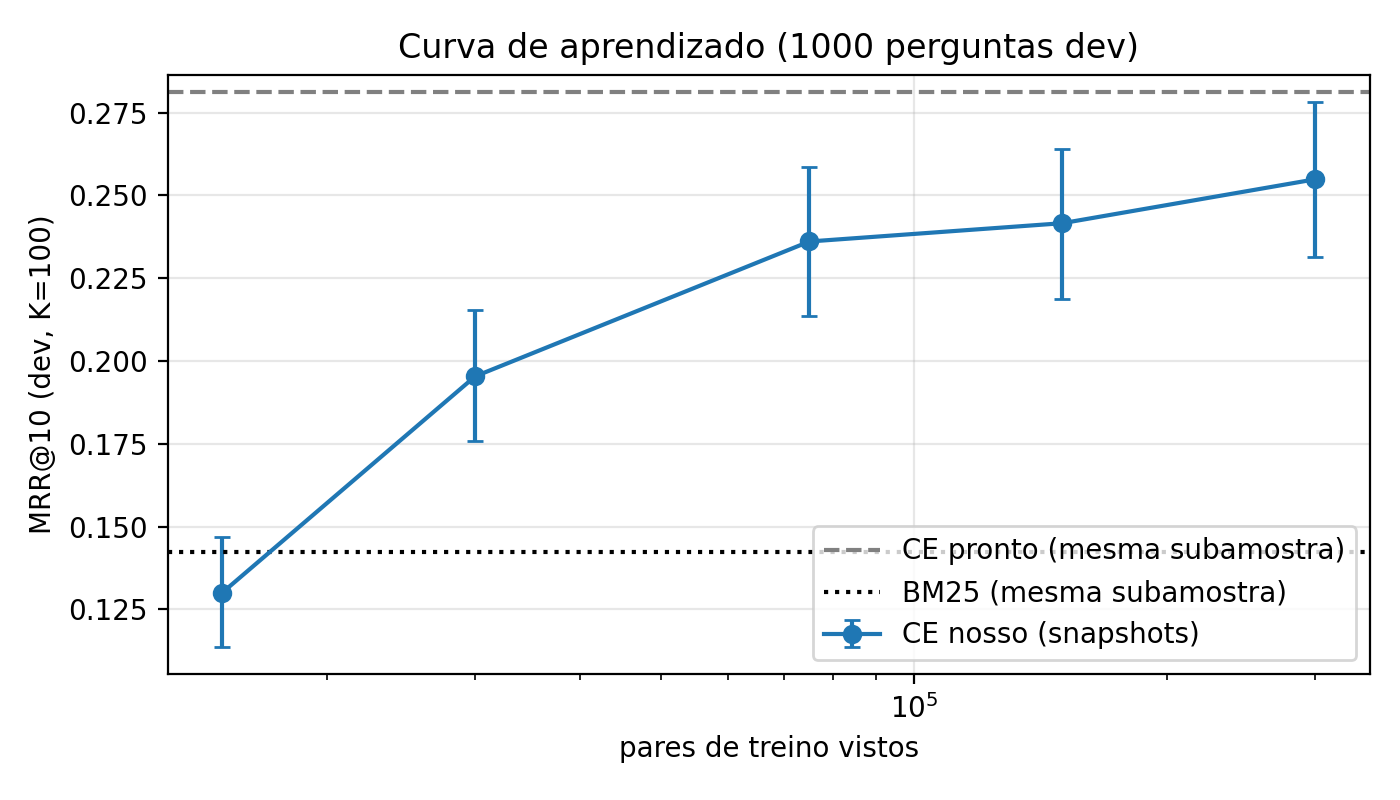
\includegraphics[width=.82\textwidth]{curva_aprendizado.png}
\caption{MRR@10 do CE nosso ao longo do treino (mil perguntas dev, IC 95\%), com o BM25 e o CE
pronto na mesma amostra.}
\label{fig:curva}
\end{figure}

\subsection{Terceiro estágio e fusão (QP3)}

\textbf{Cascata.} Sobre o CE nosso, o monoPTT5 melhora o MRR@10 em 0,021, 0,025 e 0,030 com $N$
igual a 5, 10 e 20, todos significativos. Com $N$=20, chega a 0,285, igual ao CE pronto
sozinho: um terceiro estágio forte compensa um segundo estágio mais fraco. Sobre o CE pronto,
porém, a média não muda (+0,001 a +0,002, não significativo), embora muitas perguntas mudem:
com $N$=20, 1.083 melhoram e 1.082 pioram.

\textbf{Fusão.} Esse empate, com tantas mudanças, indica que os dois modelos erram em perguntas
diferentes, e por isso combiná-los pode ajudar. A Tabela~\ref{tab:fusao} confirma: a RRF do CE
pronto com o monoPTT5 é o único ganho significativo e o melhor resultado do trabalho (0,292). As
demais combinações não ajudam:
\begin{itemize}
  \item \textbf{CE pronto + CE nosso:} os dois são o mesmo tipo de modelo, treinado no mesmo
  tipo de dado, e erram nas mesmas perguntas.
  \item \textbf{Qualquer CE + BM25:} o BM25 é muito mais fraco; a soma ponderada praticamente
  zera o peso dele.
\end{itemize}
A RRF dá o mesmo peso a todos os modelos. Isso funciona quando eles têm força parecida, mas
piorou o resultado em todos os casos com um modelo mais fraco. A soma ponderada nunca ficou
significativamente abaixo do melhor modelo isolado, porque pode simplesmente ignorar um modelo
inútil (Figura~\ref{fig:fusao}).

\begin{table}[ht]
\centering
\caption{Fusão de pontuações (MRR@10; $\Delta$ em relação ao melhor modelo isolado; $^{*}$significativo com Holm).}
\label{tab:fusao}
\small
\begin{tabular}{lccc}
\toprule
Modelos & Melhor isolado & Soma ponderada & RRF \\
\midrule
CE pronto + monoPTT5 & 0,286 & 0,290 (+0,004) & \textbf{0,292 (+0,006)$^{*}$} \\
CE nosso + monoPTT5 & 0,285 & 0,285 (+0,000) & 0,275 ($-$0,010)$^{*}$ \\
CE pronto + CE nosso & 0,285 & 0,286 (+0,000) & 0,279 ($-$0,006)$^{*}$ \\
CE pronto + BM25 & 0,285 & 0,284 ($-$0,001) & 0,232 ($-$0,054)$^{*}$ \\
CE nosso + BM25 & 0,255 & 0,252 ($-$0,003) & 0,220 ($-$0,035)$^{*}$ \\
\bottomrule
\end{tabular}
\end{table}

\begin{figure}[ht]
\centering
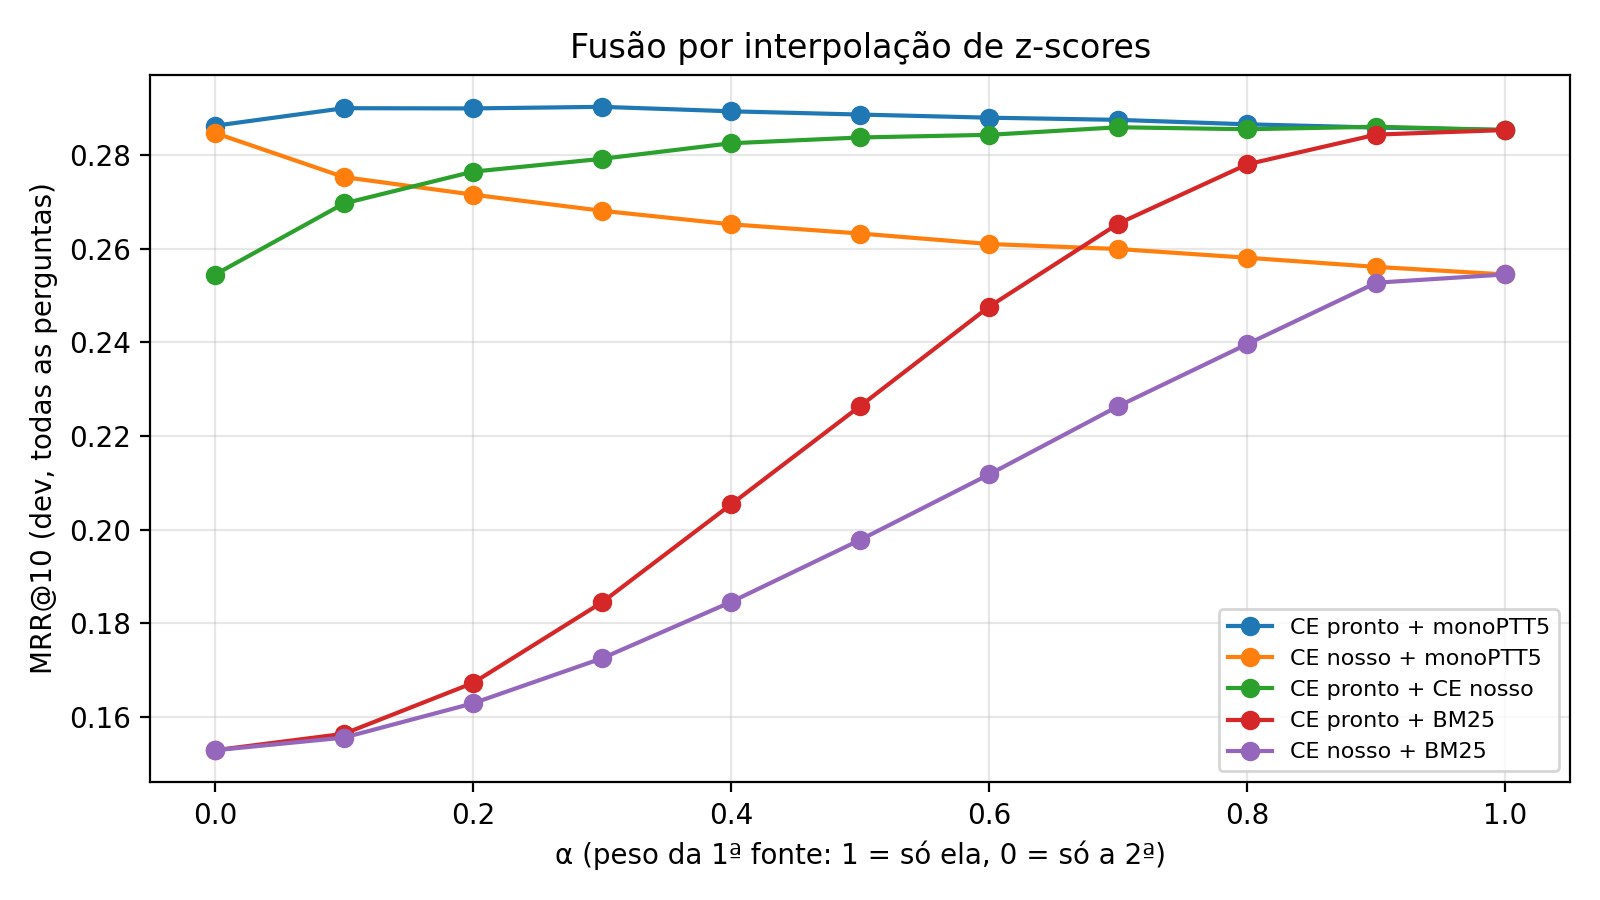
\includegraphics[width=.82\textwidth]{fusao_curva_alpha.png}
\caption{MRR@10 conforme o peso $\alpha$ do primeiro modelo na soma ponderada (1 = só o
primeiro, 0 = só o segundo).}
\label{fig:fusao}
\end{figure}

\textbf{Custo.} O monoPTT5 leva cerca de 13~ms por par, contra 1,4 a 2,4~ms do cross-encoder,
ou seja, cerca de sete vezes mais. Na amostra de mil perguntas (Tabela~\ref{tab:cascata}), a
cascata com $N$=20 tem a mesma qualidade do monoPTT5 aplicado direto ao BM25, sem diferença
significativa, gastando cerca de 36\% do tempo. Os tempos são aproximados: os dois
cross-encoders são do mesmo tamanho, mas mediram 173 e 243~ms com $K$=100, uma variação comum
em GPUs compartilhadas.

\begin{table}[ht]
\centering
\caption{Cascata contra monoPTT5 direto (mil perguntas; tempo de reranqueamento por pergunta).}
\label{tab:cascata}
\begin{tabular}{lccc}
\toprule
Sistema & MRR@10 & $\Delta$ vs direto ($p$) & Tempo (ms) \\
\midrule
CE nosso ($K$=100) & 0,255 & $-$0,036 ($<$0,001) & $\approx$240 \\
CE nosso $\rightarrow$ monoPTT5 ($N$=5) & 0,279 & $-$0,012 (0,005) & $\approx$310 \\
CE nosso $\rightarrow$ monoPTT5 ($N$=20) & 0,288 & $-$0,003 (0,077) & $\approx$500 \\
monoPTT5 direto ($K$=100) & 0,291 & --- & $\approx$1.390 \\
\bottomrule
\end{tabular}
\end{table}

\subsection{Onde o reranqueamento ajuda (QP4)}

Agrupamos as perguntas pela palavra interrogativa inicial (Tabela~\ref{tab:tipos}). O CE pronto
ganha mais em perguntas com \textit{quando} (+0,162), \textit{onde} (+0,158) e de definição
(+0,154). Nelas, a resposta (uma data, um lugar, uma explicação) quase nunca repete as palavras
da pergunta, e o BM25 vai mal. Perguntas sem palavra interrogativa, no estilo de busca por
palavras-chave, já são as mais fáceis para o BM25 (0,185) e ganham menos; as com
\textit{qual/quais} ganham menos ainda (+0,107). Perguntas curtas também ganham mais: +0,169
com até 3 palavras, contra +0,114 com 7 ou mais. Em resumo, o cross-encoder ajuda justamente
onde comparar palavras não basta.

\begin{table}[ht]
\centering
\caption{MRR@10 por tipo de pergunta (sem IC; grupos pequenos devem ser lidos com cautela).}
\label{tab:tipos}
\begin{tabular}{lcccc}
\toprule
Tipo & Perguntas & BM25 & CE pronto & Ganho \\
\midrule
\textit{quando} & 187 & 0,099 & 0,262 & +0,162 \\
\textit{onde} & 283 & 0,173 & 0,330 & +0,158 \\
definição / significado & 607 & 0,136 & 0,290 & +0,154 \\
\textit{o que} & 1.410 & 0,137 & 0,278 & +0,141 \\
\textit{quem} & 254 & 0,135 & 0,274 & +0,140 \\
palavras-chave (sem interrogativa) & 2.580 & 0,185 & 0,314 & +0,129 \\
\textit{quanto(s)} & 528 & 0,109 & 0,233 & +0,124 \\
\textit{qual / quais} & 828 & 0,137 & 0,243 & +0,107 \\
\bottomrule
\end{tabular}
\end{table}

\FloatBarrier
\subsection{Limitações}

\begin{itemize}
  \item Treino e teste são traduções automáticas; dados escritos originalmente em português
  podem dar resultados diferentes~\cite{miyaji:2026}.
  \item Há cerca de uma passagem relevante marcada por pergunta. Algumas ``derrotas'' podem
  ser passagens corretas sem marcação, então as métricas tendem a subestimar os sistemas.
  \item Treinamos uma única vez, com uma só configuração; não medimos a variação entre
  execuções.
  \item Reordenamos as 100 primeiras passagens, e não as 1.000 dos trabalhos de referência.
  \item A análise por tipo de pergunta não tem intervalos de confiança.
\end{itemize}

% =============================================================================
\section{Conclusão}
\label{sec:conclusao}

Implementamos e avaliamos cross-encoders para reordenar passagens em português. O principal
resultado metodológico é que o protocolo de avaliação muda as conclusões: perguntas de treino
e um corpus com passagens aleatórias inflaram o MRR@10 em 3,2 vezes, enquanto o protocolo
corrigido reproduz os valores publicados. Com uma GPU gratuita e 300 mil exemplos, nosso
cross-encoder alcança 77\% do ganho de um modelo publicado, e ainda estava melhorando quando o
treino terminou. Um terceiro estágio com o monoPTT5 compensa um reranqueador mais fraco, mas não
melhora um forte. Já combinar, por RRF, dois reranqueadores de força parecida e arquiteturas
diferentes dá o melhor resultado (0,292). O maior gargalo é o primeiro estágio: em 43\% das
perguntas, a resposta se perde antes do reranqueamento.

Como trabalhos futuros, propomos: treinar por mais tempo e repetir o treino com sementes
diferentes; usar as pontuações do modelo publicado para ensinar o nosso (destilação); melhorar
o primeiro estágio, por exemplo com busca densa ou mais candidatas; avaliar em dados escritos
originalmente em português; e revisar manualmente as derrotas para estimar quantas passagens
corretas estão sem marcação.

% =============================================================================
\section*{Disponibilidade do código}

O código (\textit{notebooks} do experimento preliminar e do pipeline final) e os resultados
estão em: \url{https://github.com/galax1y/nlp-reranking-mmarco-fusion}.

\section*{Declaração de uso de IA generativa}

Utilizamos o Claude Code (Anthropic, modelo Claude Opus 5.5) nas seguintes etapas: (i)
busca e organização da literatura relacionada; (ii) geração do código do pipeline final
(preparação dos dados, laço de ajuste fino, avaliação, cascata e fusão) e correção de erros;
(iii) cálculo e análise exploratória dos resultados; (iv) preparação do modelo \LaTeX{}; e (v)
redação de uma primeira versão deste texto. Todo o código e todo o texto foram revisados,
validados e reescritos pelos autores, que assumem integral responsabilidade pelo conteúdo.

\bibliographystyle{sbc}
\bibliography{references}

\end{document}
